\documentclass{beamer}
\usetheme[block=fill]{metropolis}

\usepackage{hyperref}
\usepackage{tikz}

\DeclareMathOperator{\M}{\mathcal M}
\DeclareMathOperator{\N}{\mathcal N}
\DeclareMathOperator{\G}{\mathcal G}

\newcommand{\eq}[1]{\begin{align*} #1 \end{align*}}
\newcommand{\game}[8]{\eq{\begin{array}{ccccccccc} \text{I} & #1 && #3 && #5 && #7\\ \text{II} && #2 && #4 && #6 && #8 \end{array}}}

\title[Virtual large cardinals]{Virtual large cardinals\\ {\small\textsc{European Set Theory Conference, Vienna}}}
\author[Dan Saattrup Nielsen]{Dan Saattrup Nielsen\\ University of Bristol}
\date{July 1, 2019}

\begin{document}

{
\setbeamertemplate{background canvas}{
  \tikz[remember picture, overlay]
  \node[opacity=0.4] at (9.0, -6.5){
    
\includegraphics[width = 3.0cm]{gfx/alumni.png}
    \hspace{-1.2cm}
    
\includegraphics[width = 5cm]{gfx/epsrc.jpg}
  };
}

\begin{frame}
	\titlepage
\end{frame}
}

\begin{frame}{What are they?}
  \begin{block}{Rough definition}
    A large cardinal $\kappa$ defined via \textit{set-sized} elementary embeddings is \textbf{virtual} if the elementary embeddings exist in a generic extension.
  \end{block}

  \begin{center}
    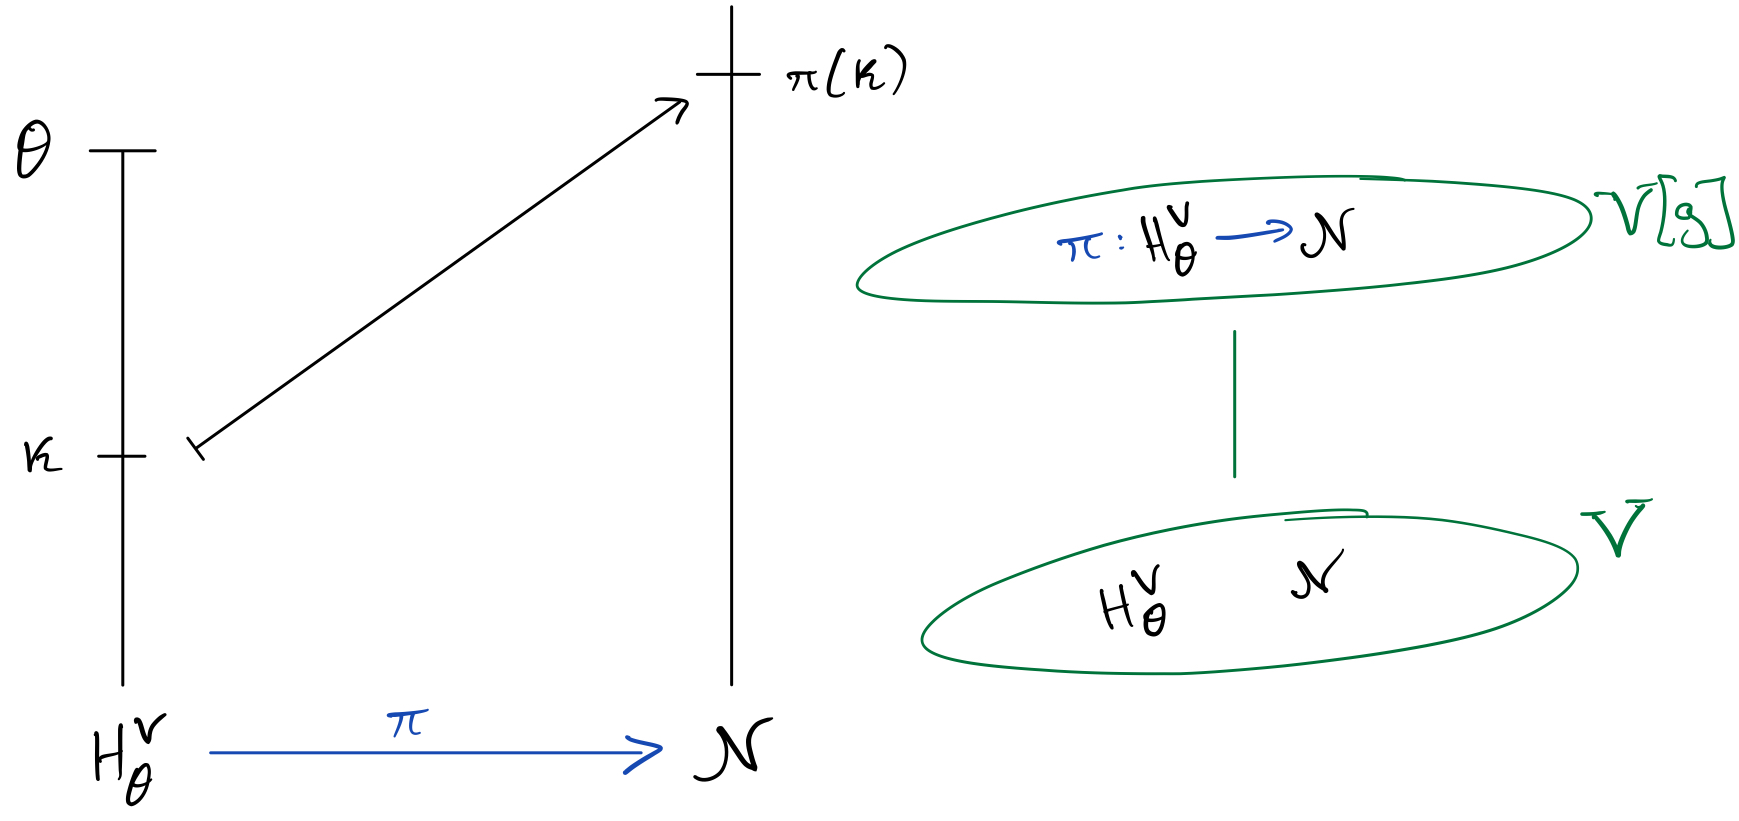
\includegraphics[scale=0.15]{gfx/virtual.jpg}
  \end{center}
\end{frame}

\begin{frame}{What are they?}
  \begin{block}{Rough definition}
    A large cardinal $\kappa$ defined via \textit{set-sized} elementary embeddings is \textbf{generic} if the elementary embeddings {\color{red} and the target model} exist in a generic extension.
  \end{block}

  \begin{center}
    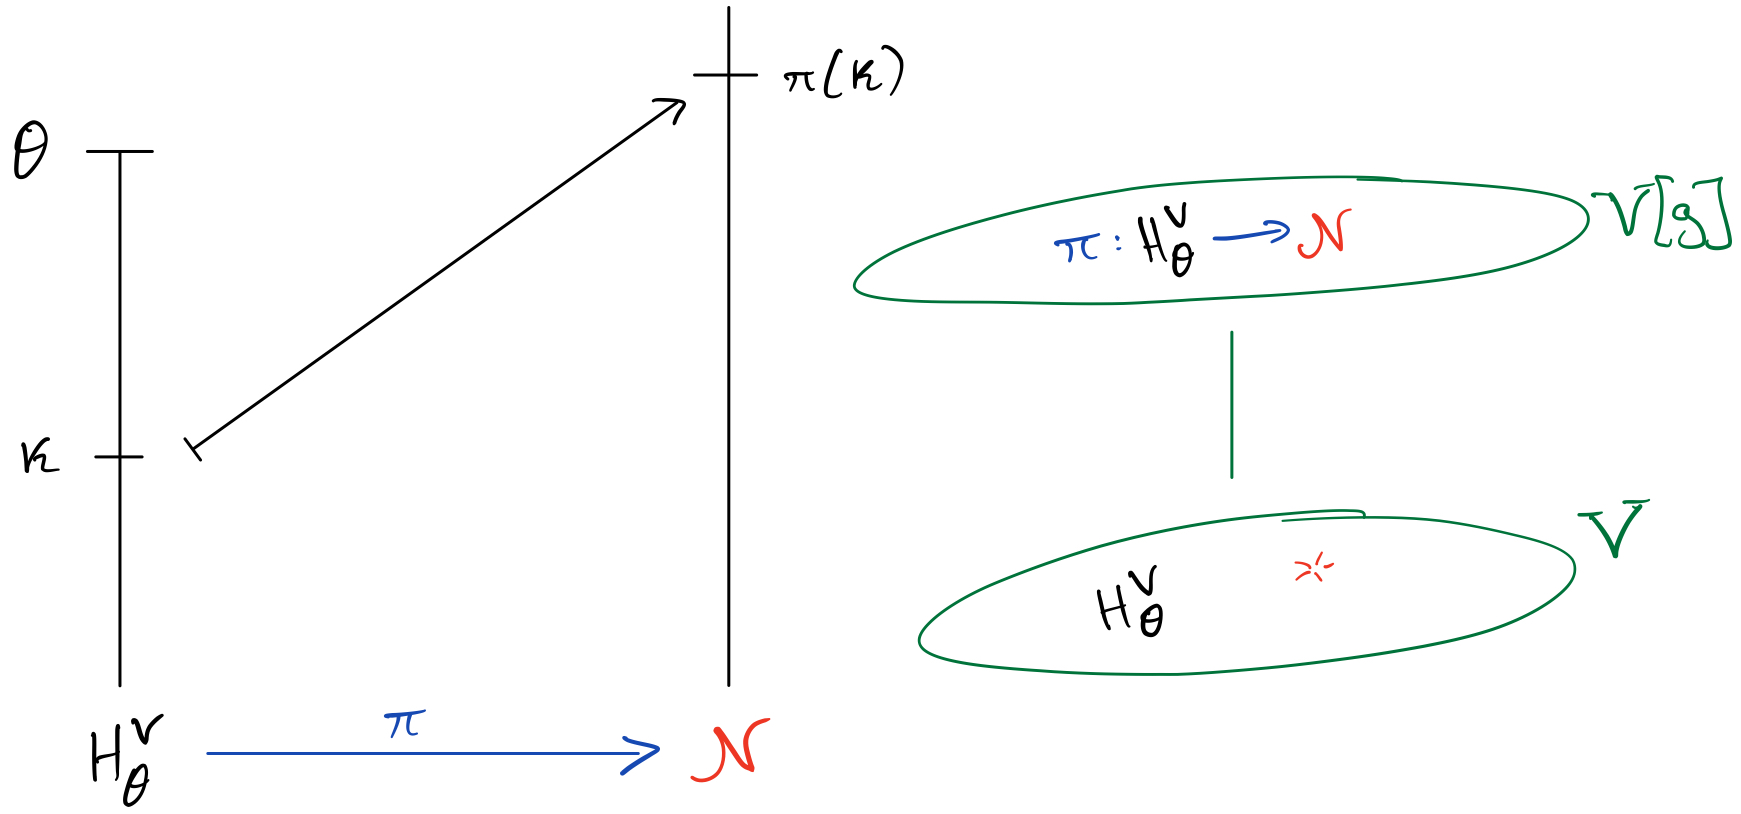
\includegraphics[scale=0.15]{gfx/generic.jpg}
  \end{center}
\end{frame}

\begin{frame}{Why should we care?}
  \begin{block}{Theorem (Schindler '00)}
    A virtually strong cardinal is equiconsistent with $\text{Th}(L(\mathbb R))$ being unchangeable by proper forcing.
  \end{block}
  
  \pause

  \begin{block}{Theorem (Schindler-Wilson '18)}
    A virtually Shelah cardinal is equiconsistent with every universally Baire set of reals having the perfect set property.
  \end{block}

  \pause
  
  \begin{block}{Theorem (Wilson '19)}
    A virtually Vop\v enka cardinal is equiconsistent with $\Theta=\omega_2$ and ${\bf\Sigma}^1_2$ being the class of all $\omega_1$-Suslin sets.
  \end{block}
\end{frame}

\begin{frame}{Where are they?}
  \begin{center}
    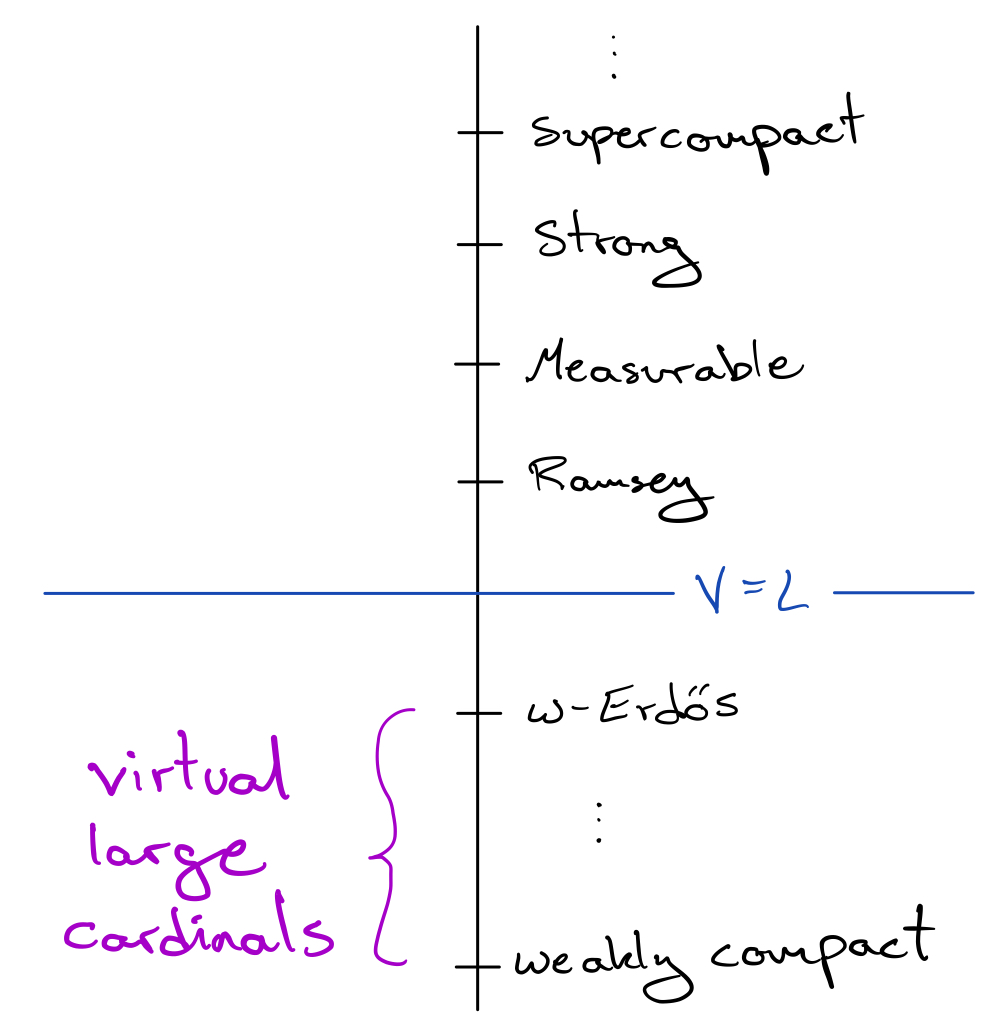
\includegraphics[scale=.16]{gfx/hierarchy.jpg}
  \end{center}
\end{frame}

\begin{frame}{How do they behave?}
  \begin{block}{Theorem (Gitman)}
    Virtually strongs are equivalent to virtually supercompacts.
  \end{block}

  \pause

  \begin{block}{Theorem (Schlicht-N.)}
    Virtually measurables are equiconsistent with virtually strongs, but they are \textit{not} equivalent.
  \end{block}
  
  \pause

  \begin{block}{Theorem (Gitman-N.)}
    Virtually Vop\v enkas are equiconsistent with \alert{prewoodins}, but they are \textit{not} equivalent.
  \end{block}
\end{frame}

\begin{frame}{Game interlude}
  \game{\onslide<2->{\alert<2>{\M_0}}}{\onslide<3->{\alert<3>{\mu_0}}}{\onslide<4->{\M_1}}{\onslide<5->{\mu_1}}{\onslide<6->{\alert<6>{\cdots}}}{\onslide<6->{\alert<6>{\cdots}}}{\onslide<7->{\M_\gamma}}{\onslide<8->{\mu_\gamma}}
  
  \begin{enumerate}
    \item \onslide<2->{$\alert<2>{\M_\alpha}\prec H_\theta$ is a $\kappa$-sized model of $\textsf{ZFC}^-$ containing $\kappa{+}1$}
    \item \onslide<3->{$\alert<3>{\mu_\alpha}$ is an $\M_\alpha$-normal $\M_\alpha$-measure on $\kappa$ such that $\text{Ult}(\M_\alpha,\mu_\alpha)$ is wellfounded}
    \item \onslide<4->{The $\M_\alpha$'s and $\mu_\alpha$'s are \alert<4>{$\subseteq$-increasing}}
    \item \onslide<5->{We take \alert<5>{unions} at limit rounds}
    \item \onslide<7->{The game lasts for \alert<7>{$\gamma{+}1$ rounds}}
    \item \onslide<8->{\alert<8>{Player II wins} iff they can continue playing all rounds}
    \item \onslide<9->{\alert<9>{\textsc{Important remark:}} The $\mathcal M_\alpha$'s are \textbf{not} necessarily transitive!}
    \item \onslide<10>{This game is called $\alert{\G_\gamma^\theta(\kappa)}$. If we restrict I to only add ${<}|\gamma|$ sets at a time then we call the game $\alert{\mathcal{C}_\gamma^\theta(\kappa)}$.}
  \end{enumerate}
\end{frame}

\begin{frame}{How do they behave level by level?}
  \begin{block}{Theorem (Schindler-N.)}
    $\kappa$ is generically $\theta$-measurable iff II wins $\mathcal{C}_\omega^\theta(\kappa)$.
  \end{block}
   
  \pause

  \begin{block}{Theorem (Schindler-N.)}
    If $\kappa$ is virtually $\theta$-\alert{prestrong} then II wins $\G_\omega^\theta(\kappa)$, and if II wins $\G_\omega^\theta(\kappa)$ then $\kappa$ is generically $\theta$-\alert{power}-measurable.
  \end{block}
\end{frame}

\begin{frame}{How do they behave level by level?}
  \begin{center}
    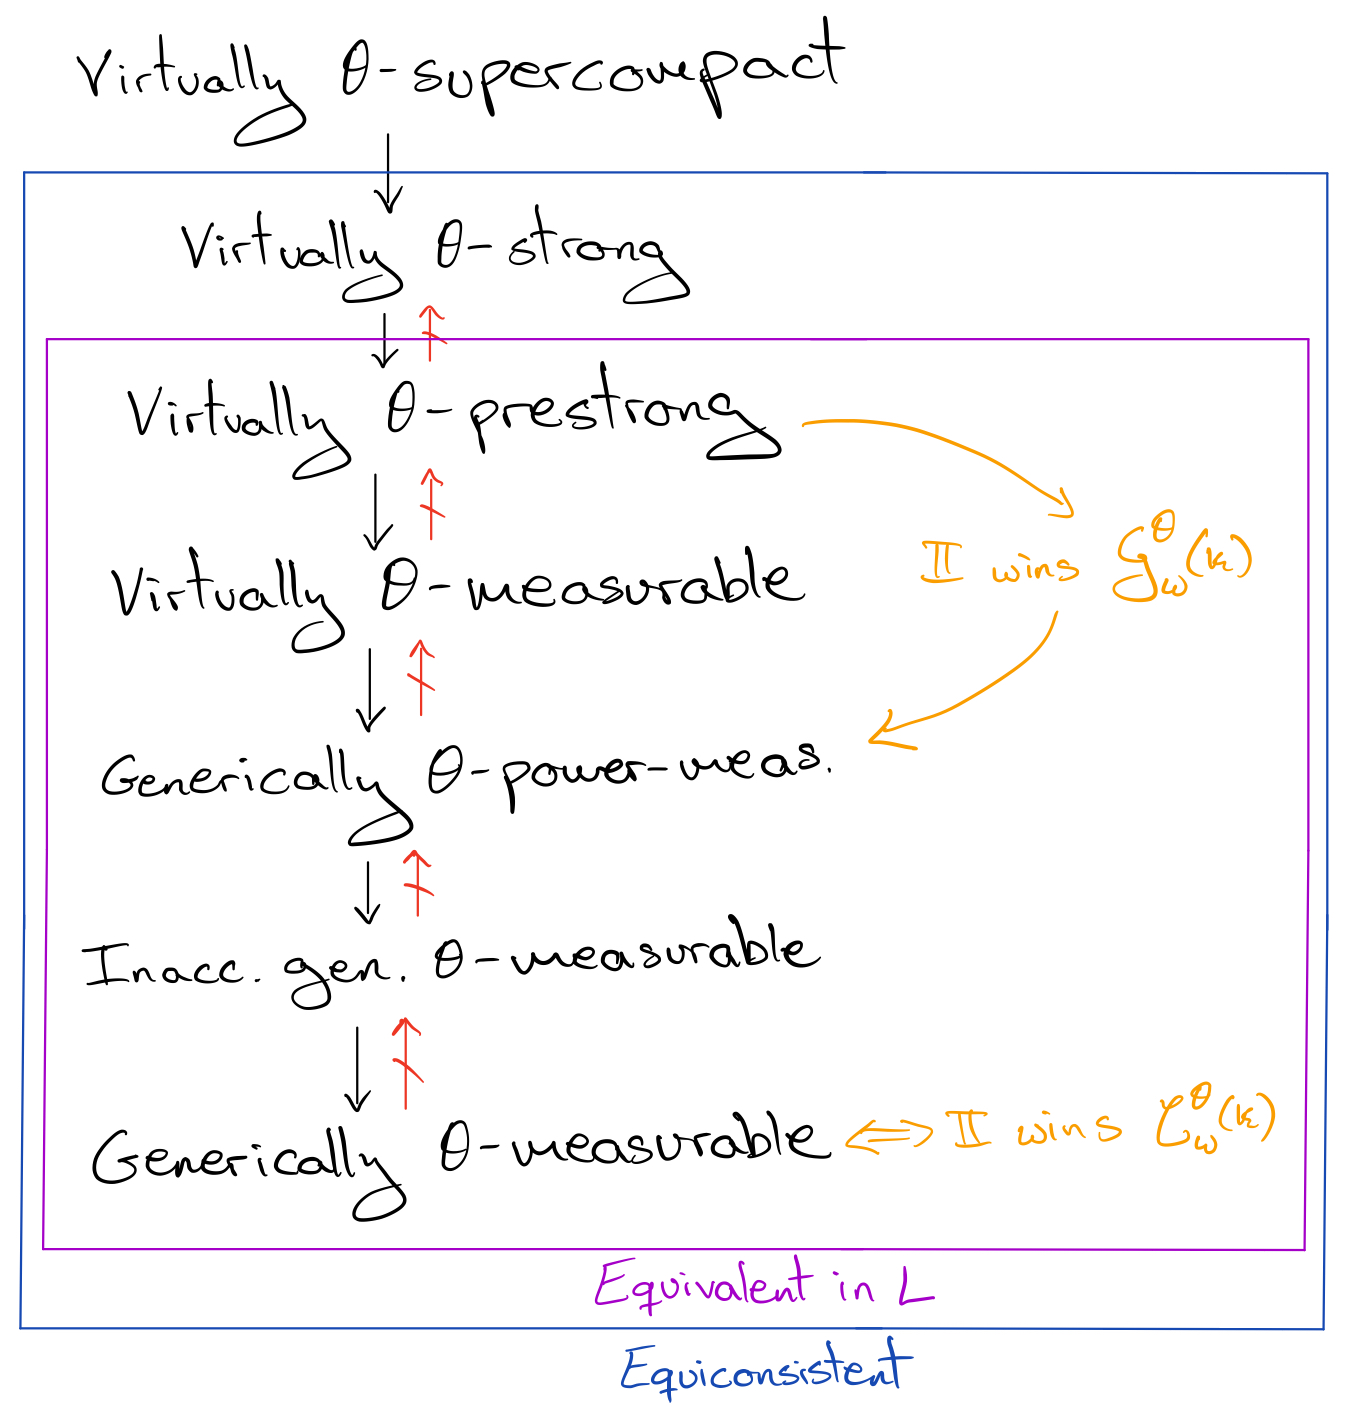
\includegraphics[scale=.16]{gfx/lbl_virtual.jpg}
  \end{center}
\end{frame}

\begin{frame}{Future work}
  \begin{enumerate}
    \item Are virtually $\theta$-strongs equivalent to virtually $\theta$-supercompacts?
    \pause\item Level-by-level behaviour in larger core models?
    \pause\item Game characterisations of other generic large cardinals?
    \pause\item Virtualising small embedding cardinals like Ramsey cardinals and below?
    \pause\item Indestructibility properties?
  \end{enumerate}
\end{frame}

\begin{frame}{}
  \begin{center}
    {\Large Thank you for your attention.}
  \end{center}
\end{frame}

\end{document}
